%!TEX root = ../thesis.tex
\chapter{Design \& Implementation}

	Development of a graphical user interface for libmapper creates a unique challenge. Obviously such an interface is a practical tool, and should function as such, yet it also must work in concert with DMIs which are inherently designed for creative use. For the purposes of this project, the assumed solution to this innate paradox is to provide the user with multiple independent modes of control.  libmapper itself is an extremely flexible API that makes few assumptions as to the network of devices and signals or how they are mapped. It is thus fitting that a GUI for libmapper would be equally as flexible. In lieu of a single perfect solution for network visualization and interactivity, providing users with various independent views offered good compromise.

	Work on MapperGUI began with the Webmapper interface described in section \ref{sub:webmapper}. An MVC structure was built around the code to make the program more extensible and to allow for the easy integration of multiple views. Missing features from Maxmapper were incorporated into the main view mode, ListView. ListView was extended in various ways, taking advantage of the new code base. Two new view modes, GridView and HiveView,\footnote{Both designed by Jonathan Wilansky at IDMIL} were then integrated into the main GUI. Finally, the code was compiled together as a standalone application, ready for wide distribution.

%%%%%%%%%%%%%%%%%%%%%%%%%%%%%%%%%%%%%%%%%%%%%%%%%%%%%%%%%%%%%%%%%%%%%%%%%%%%%%%%%%%%%%%%%%%%%%%%%%%%%%%%%%%%%%%%%%%%%%%%%%%%%%%%%%%%%%%%%%%%%%%%%%%%%%%%%%%%%%%%%%%%%%%%%%%%%%%%%%%%%%%%%%%%%%%%%%%%%%%%%%%%%%%%%%%%%%%%%%%%%%%%%%%%%%%%%%%%%%%%%%%%%%%%%%%%%%%%%%
\section{Development of a Flexible System} % (fold)
\label{sec:development_of_a_flexible_system}

Prior GUIs for libmapper have been used successfully for some time, but all have failed to become a standard for the same reason: they cannot accommodate all possible use-cases of libmapper. List based views like Maxmapper and Webmapper cannot show hierarchies while the cluster view implemented in Vizmapper can be overly cumbersome for interaction with simple networks. With so much work already completed on prior GUIs, it was more suitable to integrate different approaches into a single GUI, rather than to begin work on some new, hopefully superior approach that would likely prove to be flawed like all that came before. 

MapperGUI integrates multiple interfaces simply: via a drop-down menu on the upper corner of the window. Options on this menu represent available visualization modes. By selecting a new visualization mode the GUI drastically changes its appearance, replacing nearly every visual element in the display.
	%Needs to be adaptable, show any metadata

	\subsection{MVC architecture} % (fold)
	\label{sec:mvc_architecture}

Because we require a modular design, the Model-View-Controller (MVC) architecture\footnote{Described in section \ref{sec:mvc_background}.} was used as a general framework for structuring the application. In fact, the whole-scale swapping of independent visual modes is a very straightforward implementation of MVC. Unfortunately, the \url{libmapper} $\rightarrow$ \url{python monitor} $\rightarrow$ \url{browser} implementation complicates matters slightly.\footnote{Compare figure \ref{fig:mapper_network} with (TODO).} A few layers of abstraction are added to take into account the monitor, the network itself and control features independent to the view (see section \ref{sec:top_toolbar}), but the general MVC architecture is maintained.

\begin{figure}
\centering
	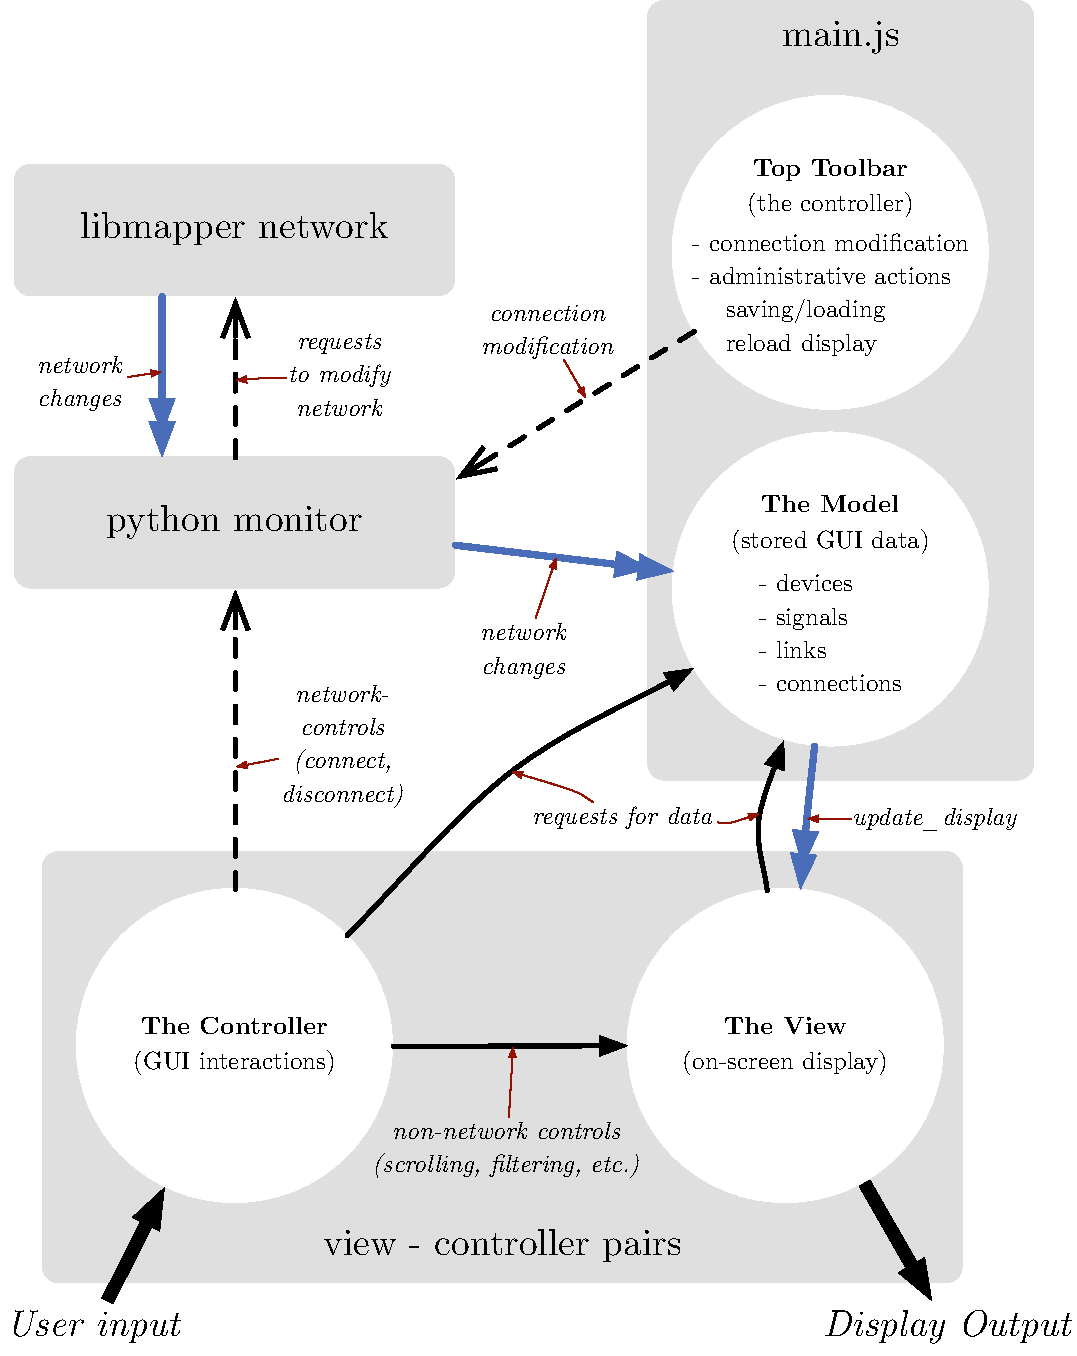
\includegraphics[width=0.9\textwidth]{figures/mapper_network}
\caption{Structure of MapperGUI. Blue arrows show propagation of network changes, dashed arrows denote messages requesting a network change.}
\label{fig:mapper_network}
\end{figure}


		\subsubsection{Independent communication}

First and foremost, it is essential that data on the screen reflect data on the network. This is not entirely straightforward, as asynchronous messages are constantly relayed between MapperGUI and libmapper. In a truly distributed system, data on the libmapper network changes continuously as other users add devices and modify mappings. Our system insulates the actual libmapper network, the displayed data and user interaction elements from one another (figure \ref{fig:mapper_network}). For example, a user command to link the two devices \url{source.1} and \url{dest.1} will send the following message to the python monitors:

\url{ {"cmd":"link","args":["/source.1","/dest.1"]} }

Meaning: a linking command is sent to \url{source.1} and \url{dest.1}.\footnote{The message itself is a python dictionary.} After this, the display does not change, as it has not yet been notified of a new link. The monitor then relays this message to the libmapper network. If the link is successful, the monitor receives notice, and sends a message to the main JavaScript file (main.js):

\url{("new_link", {"src_name": "/source.1", "dest_name": "/dest.1"}) }

This states that a new link has been formed between the source device \url{source.1} and the destination device \url{dest.1}. Only then does the GUI respond to the change on the network. Signal data itself is not available to MapperGUI in any way, as libmapper networks are designed to prevent this kind of bandwidth clutter \shortcite{new_libmapper}.

		\subsubsection{The model}

The model consists of an abstract copy of the network residing on the local machine. Independent views can consult these data, but cannot directly modify it. Messages from the python monitor announce new links, modifications to connections, or any other changes on the network. The model records these changes into four data structures:

\begin{itemize}
 	\item \url{model.devices}: Storage of all present devices and device metadata.
 	\item \url{model.links}: A record of all links on the network.
 	\item \url{model.signals}: Monitors signals on the network, but only signals that are currently visible in the GUI. This is done to save bandwidth and processing power. 
 	\item \url{model.connections}: All connections and connection metadata between signals currently in the model.
 \end{itemize} 

It is possible that previously viewed signals will persist in the model, but their connections not be updated.

		\subsubsection{View-controller pairs}

All interaction handlers\footnote{Responses to mouse clicks and keypresses.} and visualizations are stored in modular, view-controller pairs, as recommended by \citeN{MVC_krasnerpope}. Each view-controller pair corresponds with a single view mode. Pairs can have any combination of UI handlers and visual features, but must have the following four functions:

\begin{itemize}
	\item \url{view.initialize()}: Calls upon the view to create its visual elements and add its individual interaction handlers.
	\item \url{view.get_focused_devices()}: Returns whichever devices are currently visible in the view. This is used for populating the \url{model.signal} and \url{model.connection} data structures, as well as for saving and loading.
	\item \url{view.cleanup()}: Causes the controller to remove all interaction handlers.
	\item \url{view.update_display()}: Called whenever the model changes. The view is not made explicitly aware of \emph{what} has changed, but only that a change has occurred. In each view mode, this call causes visual features to be cleared and re-drawn. Though this creates more processor overhead (see section \ref{sec:testing_program_responsiveness}), it allows for much greater flexibility in designing new views. The model does not need to be aware of any specific informational requirements for each view.
\end{itemize}

	% subsection mvc_architecture (end)

	\subsection{Top toolbar} % (fold)
	\label{sec:top_toolbar}

It is sensible to include certain tasks and information providing structures across visualization modes. In light of this, a single view-controller pair runs continuously in MapperGUI in the form of a toolbar at the top of the window. As a part of the code structure, it communicates independently with the monitors and other view-controller pairs. This toolbar contains all administrative controls and connection modification fields. 

\begin{figure}[!ht]
\centering
	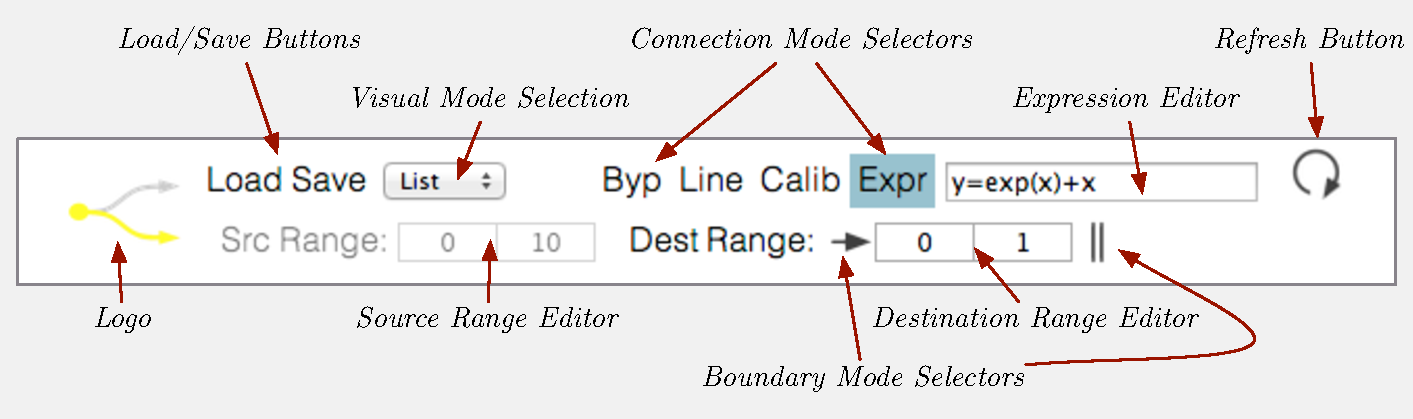
\includegraphics[width=1\textwidth]{figures/top_toolbar}
\caption{The upper toolbar}
\label{fig:toolbar}
\end{figure}

\begin{itemize}
	\item \textbf{Administrative controls}
	\begin{itemize}
		\item\emph{Load/Save buttons}: These elements respond to clicks to save and load mappings, as discussed in section \ref{sec:saving_and_loading}.
		\item\emph{Visual mode selection}: A drop-down menu containing all view modes for user selection.
		\item\emph{Refresh Button}: When clicked, all data residing on the model is erased and re-gathered. This is useful if the monitor somehow desynchronizes with the network.
	\end{itemize}

	\item \textbf{Connection modification}: The following controls are only available when the user selects a single connection.
	\begin{itemize}
		\item\emph{Connection mode selectors}: An array of buttons allowing the user to choose between available connection modes.
		\item\emph{Expression editor}: Here the user can input a custom expression if the selected signal is in the \emph{Expression} mode. In other connection modes this field displays the connection's expression but is not editable.
		\item\emph{Source range editor}: These two numbers display the maximum and minimum values of the input signal. These fields is only editable in the \emph{Line} connection mode.
		\item\emph{Destination range editor}: Same as above but for destination signals. Due to boundary conditions these fields are useful in all modes.
		\item\emph{Boundary mode selectors}: Two buttons that cycle through the five boundary modes for the maximum and minimum destination values. A small graphic represents each mode.
	\end{itemize}
\end{itemize}

All interface features not present in the top toolbar are part of the current visualization mode and reside in a ``container'' element below, occupying the remainder of the window.

	% subsection top_toolbar (end)

The file and communication structure described in this section allows for quick modification and extension of the interface. Developers can program new visual modes relatively easily, in comparison to prior GUIs. Hopefully this will eventually lead to a GUI with many useful view modes that can accommodate nearly every use-case for libmapper.

% section development_of_a_flexible_system (end)

%%%%%%%%%%%%%%%%%%%%%%%%%%%%%%%%%%%%%%%%%%%%%%%%%%%%%%%%%%%%%%%%%%%%%%%%%%%%%%%%%%%%%%%%%%%%%%%%%%%%%%%%%%%%%%%%%%%%%%%%%%%%%%%%%%%%%%%%%%%%%%%%%%%%%%%%%%%%%%%%%%%%%%%%%%%%%%%%%%%%%%%%%%%%%%%%%%%%%%%%%%%%%%%%%%%%%%%%%%%%%%%%%%%%%%%%%%%%%%%%%%%%%%%%%%%%%%%%%%
\section{Integration of Interface Features} % (fold)
\label{sec:integration_of_interface_features}

Development began by unifying features of the Maxmapper onto the Webmapper code. Webmapper was selected as a starting point because of cross-platform nature of a web-based implementation. The general two-table structure of Maxmapper and Webmapper created the first view mode of the interface, ListView.

	\subsection{Structure of ListView} % (fold)
	\label{sub:ListView}

Of all currently available views, ListView provides the most straightforward way to visualize and interact with libmapper. Two tables dominate the visible area listing source elements on the left and destination elements on the right. B\'ezier curves sit on a central canvas and form lines between associated list elements on each each side. Because these curves do not always represent the same data structure, the lines themselves are referred to as \emph{arrows} by the GUI code and by this document.

\begin{figure}[ht]
\centering
	\scalebox{0.4}{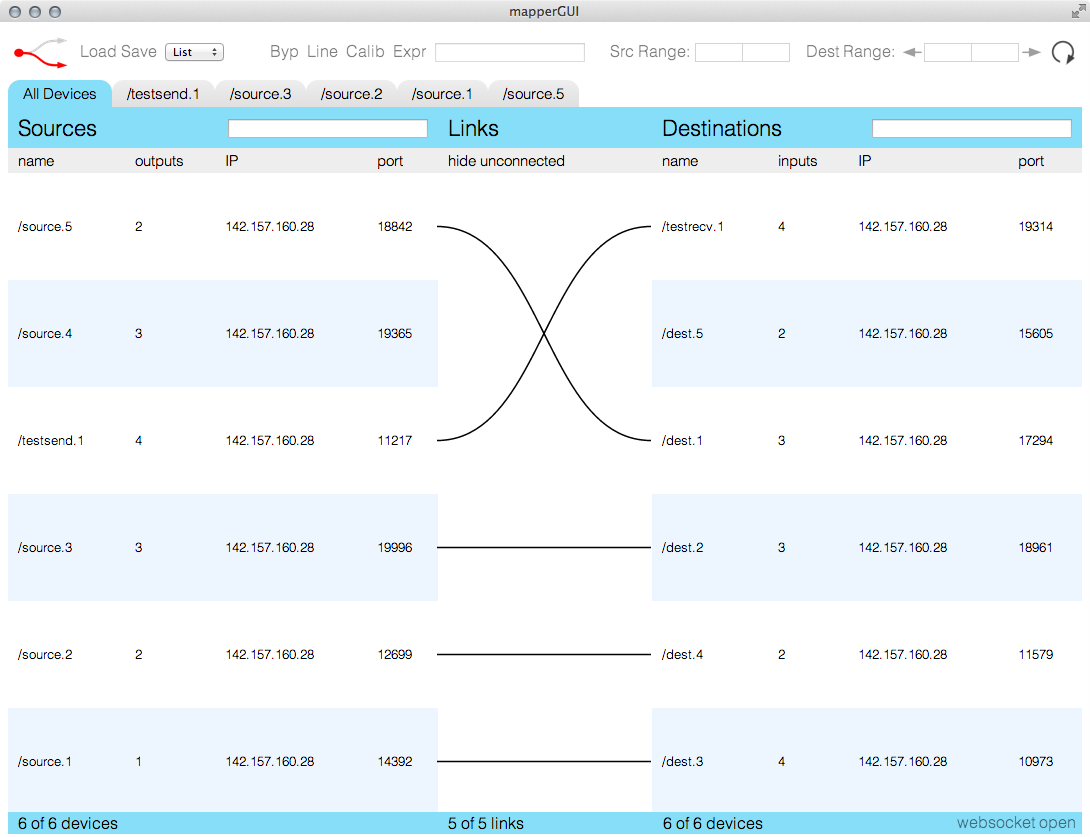
\includegraphics{figures/list_view_all_devices}}
\caption{The list view with all devices selected}
\label{fig:list_view_all_devices}
\end{figure}

The view itself is divided into two major modes: ``All Devices'' and groups of signals. Switching between these modes is accomplished through tabs that appear at the top of the container, much like the tabs in modern web browsers. In the All Devices tab, ListView lists network devices, as in figure \ref{fig:list_view_all_devices}. Source devices inhabit the left table, while the right table lists destination devices. Intermediate devices\footnote{Devices with both inputs and outputs, such as implicit mappers described in \citeN{interpolated_mappings}.} will be listed in both tables. The view displays device metadata as columns of each table. Here arrows represent links between devices. Since no connections or signals are shown, most of the top bar (see section \ref{sec:top_toolbar}) is disabled in the All Devices tab. Saving and loading are also disabled.

\begin{figure}[ht]
\centering
	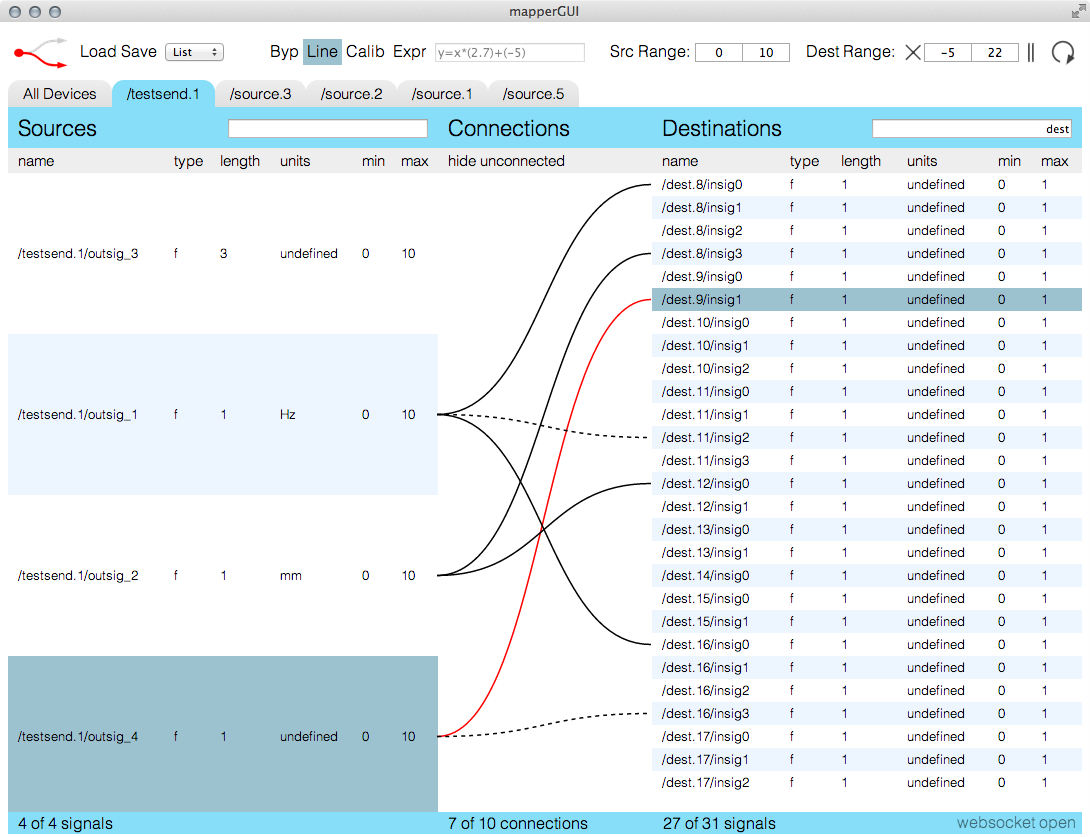
\includegraphics[width=1\textwidth]{figures/list_view_single_link}
\caption{The list view with device \textbf{testsend.1} selected}
\label{fig:list_view_single_link}
\end{figure}

MapperGUI draws a tab for every source device with at least one link to a destination device. Clicking on any of these tabs will redraw both tables. The left table now shows all child signals for the selected source device while the right table displays child signals for every destination device linked to that source. In this mode arrows represent connections which can be modified using the top toolbar.

	% subsection ListView (end)
	
	\subsection{Display libmapper metadata} % (fold)
	\label{sub:display_libmapper_metadata}

Tables in the original Webmapper interface have no headers. Without these queues, only a small amount of metadata is provided (see figure \ref{fig:webmapper}).

\begin{table}
	\centering
	\Tcaption{Metadata available in Webmapper vs list view}
	\label{tab:webmapper_list_view_metadata}
		\begin{tabular}{l  l  |  l l }
		\hline\hline
		\textbf{webmapper}&&\textbf{list view}\\
		Devices&Signals&Devices&Signals\\
		\hline
		name&name&name&name\\
		IP address&data type&IP address&data type\\
		port&vector length&port&vector length\\
		&&number of inputs&units\\
		&&number of outputs&maximum value\\
		&&&minimum value\\
		\end{tabular}
\end{table}

Incorporating a useful feature of Maxmapper, column headers have been added to the ListView. Also included are new pieces of device and signal metadata, as listed in table \ref{tab:webmapper_list_view_metadata}. Tables draw themselves with invisible extra columns, such that adding extra data can be easily accomplished. If a user embeds extra metadata onto devices or signals that data will automatically include itself in the display.  

In general, MapperGUI tries to keep possible extensions like this to libmapper in mind. Very little is assumed about the network itself. In turn, the only device metadata that \emph{must} exist is the device name and number of inputs/outputs, MapperGUI uses to place the device in either the source or destination table. For signals, MapperGUI takes vector length into account when deciding whether two signals are compatible and can be connected. However, dis-including length in the signal metadata will not result in an error.
	
	% subsection display_libmapper_metadata (end)

	\subsection{Locating devices and signals} % (fold)
	\label{sub:locating_devices_and_signals}

In networks with dense arrays of devices or signals, it can be difficult to find particular objects. Three features from Maxmapper were adapted for use with ListView to aid in such tasks.

First, regular expression\footnote{TODO} supporting search-bars are now present at the top of each table. If the user types an expression of any kind into either of these fields, ListView will filter elements displayed in the table beneath. Table rows can be filtered not just by the names of the signals/devices, but also by length, units, IP address or any other piece of information in the table row. To make the filter more responsive the filtration code runs with every keypress such that the table is dynamically modified as the user inputs characters to the search field. 

A common use-case for Maxmapper was a large list of signals with only a handful of connections that needed constant modification. Obviously scrolling through a list with hundreds of rows, only to repeatedly select between the same handful of connections can be very tedious. To assist these users Maxmapper features a ``hide-unconnected'' button that was incorporated into ListView as well. The button sits in a previously unused piece of screen above the central canvas (see figures \ref{fig:list_view_all_devices} and \ref{fig:list_view_single_link}). When clicked, the GUI hides all signals not currently connected to any others. The text on this button then changes to ``show-unconnected.''

\begin{figure}
	\centering
	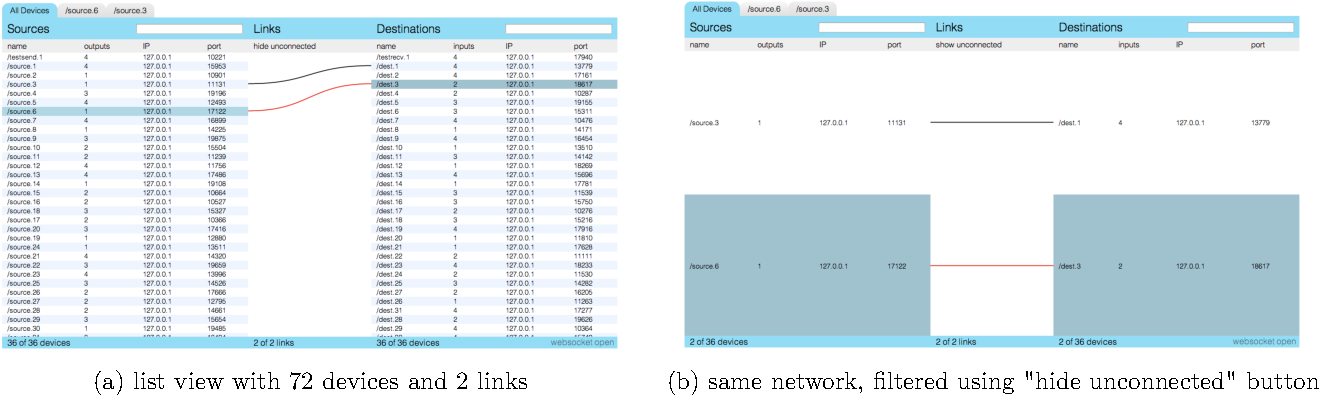
\includegraphics[width=1\textwidth]{figures/hide_unconnected}
\caption{Functionality of hiding unconnected elements on a network with many devices and few links.}
\label{fig:hide_unconnected}
\end{figure}

Finally, tables can sort themselves by individual columns. Signals and devices are initially placed into the table in whichever order they appear in the model. Upon a click to any column header, the table sorts the information ``descending'' (first numerically, then alphabetically) by that column. A second click on the same header will re-sort the information in an ``ascending'' fashion. Users can sort table rows by any metadata appearing in the table.

	% subsection locating_devices_and_signals (end)

	\subsection{Visual feedback} % (fold)
	\label{sub:visual_feedback}

User feedback was a very important part of the design process (see section \ref{sec:user_feedback}). One observation re-iterated by nearly all users of MapperGUI and prior GUIs was that it became extremely frustrating when the display became out of sync with the network, or when it seemed like the GUI \emph{might} be out of sync. To ameliorate these difficulties, MapperGUI incorporates a few Maxmapper features entirely for visual feedback.
		
		% # of signals/etc.
At the very bottom of the window is a bar displaying the number of features on the network versus the number currently visible. For example, if there are 36 source devices on the network, but the user has filtered out all but two, then the field underneath the source table will read ``2 of 36 devices'' (as in figure \ref{fig:hide_unconnected}). These data are also shown for destination devices, links, connections and signals. This is done in order to help the user diagnose technical problems. If a desired signal does not appear, perhaps the device has become unresponsive or the user has encountered an error in MapperGUI. If the user has simply filtered out the signal somehow, it is much more straightforward to see this immediately than to begin searching for possible technical problems.\footnote{libmapper and MapperGUI are both at a stage of development where bugs are an inevitable part of the user experience. We like to call them ``features.''}

		%top toolbar, muting
The top toolbar automatically reflects metadata for selected connections. Expressions, connection modes and ranges can be observed simply by clicking on the arrow representing a connection. The toolbar displays non-editable fields (depending on connection mode) as slightly more transparent. Arrows are re-drawn with dashed lines for muted connections, as in figure \ref{fig:list_view_single_link}.

		% row striping
Though not feedback on the network itself, large tables are more easily navigable when rows have ``zebra'' striping. The display re-calculates this alternate row striping any time a user filters the view. Rows highlight themselves when selected. Any number of rows on either table can be selected simultaneously. Row highlighting works in combination with row striping (see figure \ref{fig:row_striping}).

\begin{figure}[!h]
	\centering
	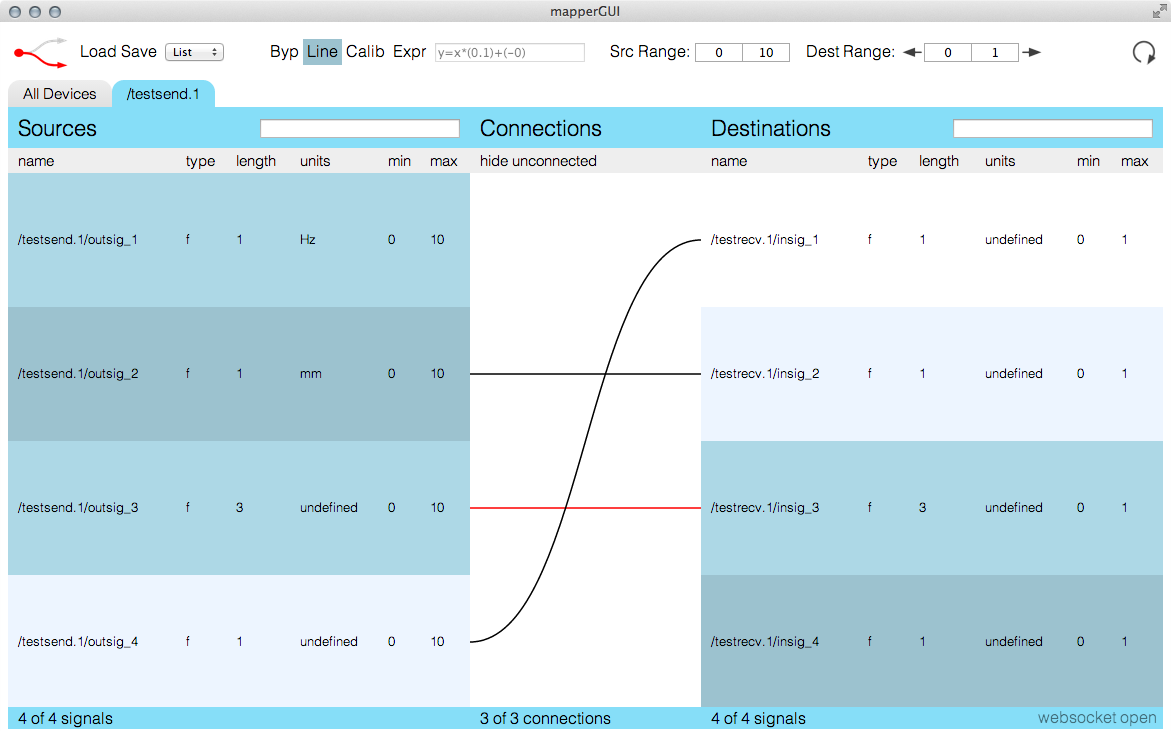
\includegraphics[width=1\textwidth]{figures/row_striping}
	\caption{Multiple selection and row striping in ListView.}
	\label{fig:row_striping}
\end{figure}

By incorporating popular visual feedback elements from Maxmapper, we were able to make the display more robust and useful. Though difficulties with interaction can still occur (missing devices, unresponsive connections, etc.), good visual feedback should allow users to more quickly diagnose and solve these problems.

	% subsection visual_feedback (end)

	\subsection{Improvements to User Interaction} % (fold)
	\label{sub:improvements_to_user_interaction}

Easily the greatest user complaint about Webmapper was the nature of its interaction. In order to form a connection, a user must click on a source device, then a destination device, then finally click a ``connect'' button. Even for simple mappings this was seen as overly cumbersome. In order to make MapperGUI useful, we clearly needed to improve on the speed of interaction. Fortunately UI features in Maxmapper helped solve this problem.
	
		\subsubsection{Draggable links and connections}

The drag to connect gesture is common among similar interfaces (\citeNP{patchage}, \shortciteNP{integra}), and is featured in Maxmapper as well. Though more advanced to program than the improvements listed above, it was seen as necessary to get libmapper users to switch to from Maxmapper to our GUI.

\begin{figure}[h]
	\centering
	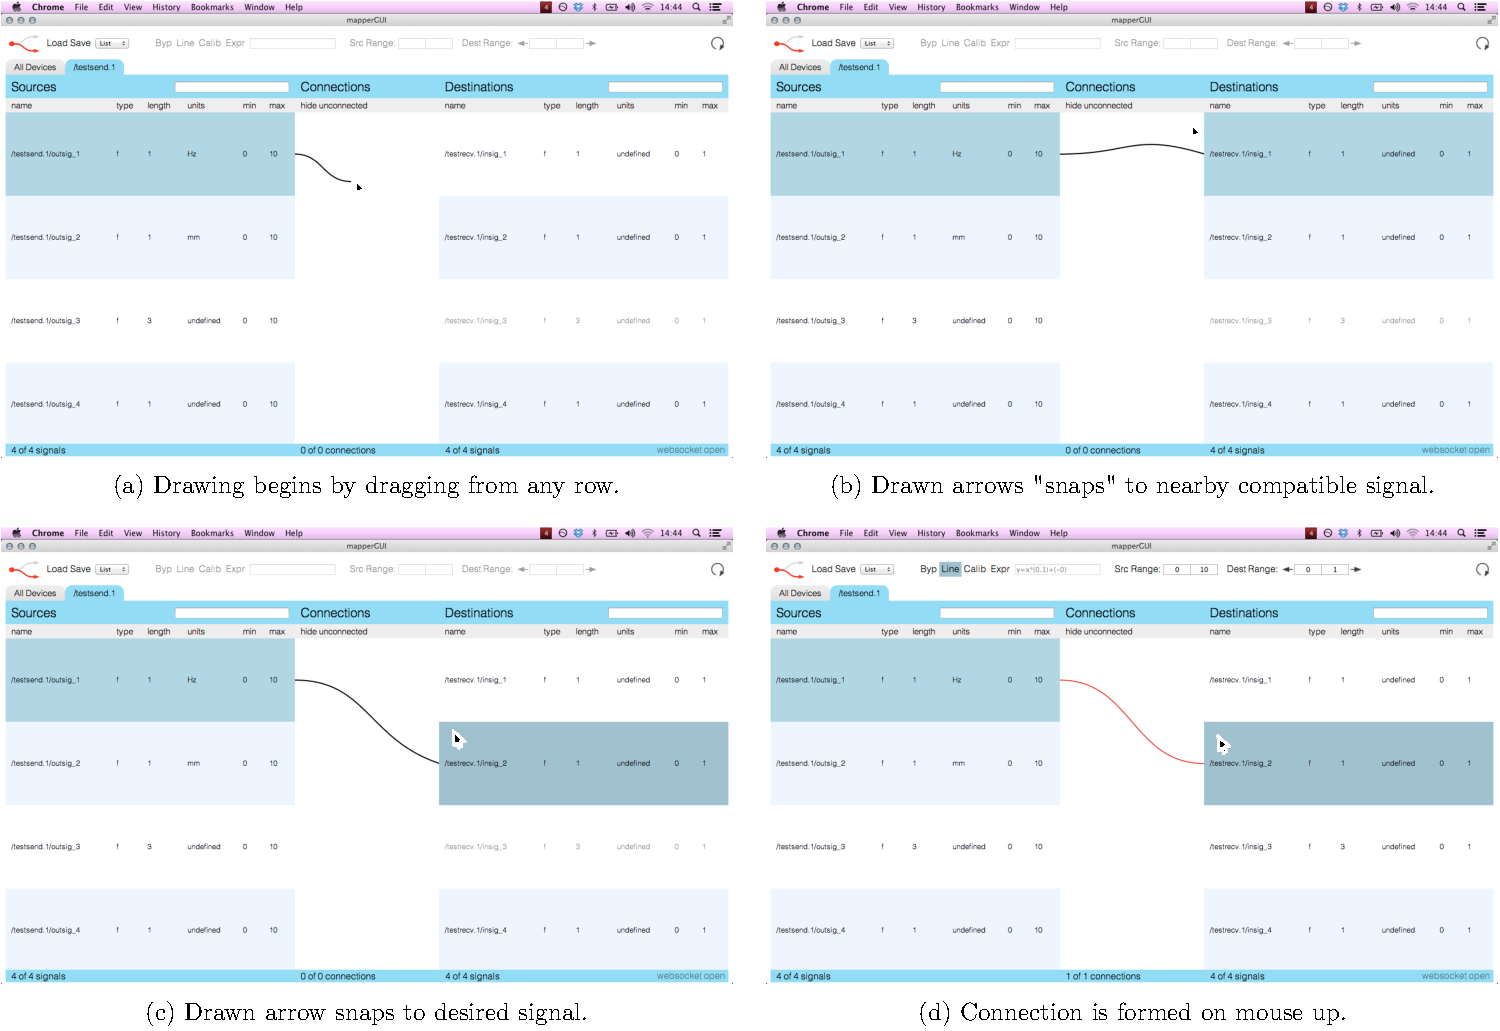
\includegraphics[width=1\textwidth]{figures/drawing}
	\caption{Draggable links and connections.}
	\label{fig:drawing}
\end{figure}

The user can click on any table row and drag onto the central canvas. Upon doing so, a slightly-thicker B\'ezier curve begins to follow the mouse pointer about the canvas. Incompatible signals become transparent. Once the mouse pointer comes within 50 pixels of the other table the drawn arrow snaps to the nearest row if it is compatible, highlighting that device or signal. The user then can scroll the mouse up and down the rows of the target table and the drawn arrow will continue snapping to the nearest available row. Once the user lifts up on the mouse button, MapperGUI sends a message to libmapper asking either connect the appropriate signals or to link the appropriate devices.

Of course, ListView does not draw the final linking/connecting arrow until a confirmation message is received from the monitor, by way of libmapper itself. Figure \ref{fig:drawing} demonstrates a dragged connection starting from a source signal and ending on a destination signal, though the same gesture is possible beginning with destination elements.

	%also possible to drag right to left

		\subsubsection{Keyboard shortcuts}

To further accelerate GUI operations, some keyboard shortcuts were added:

\begin{table}[!h]
	\centering
	\Tcaption{Shortcut keys in ListView}
	\label{tab:list_view_shortcut_keys}
		\begin{tabular}{l  l  l}
		\hline\hline
		key combination&action&from Maxmapper?\\
		\hline
		c 					& Connect/link selected rows & no\\
		delete 				& Disconnect/unlink all selected & yes\\
		command + a 		& Select all visible connections/links & yes\\
		alt + tab 			& Change tab to the right & no\\
		alt + shift + tab 	& Change tab to the left & no\\ 
		m 					& Mute all selected connections/links & yes\\
		\end{tabular}
\end{table}

For PC users, the ``select all'' key command is ``control + a.'' Tab changing is meant to further mimic functionality of web browsers. 

	% subsection improvements_to_user_interaction (end)

% section integration_of_interface_features (end)

%%%%%%%%%%%%%%%%%%%%%%%%%%%%%%%%%%%%%%%%%%%%%%%%%%%%%%%%%%%%%%%%%%%%%%%%%%%%%%%%%%%%%%%%%%%%%%%%%%%%%%%%%%%%%%%%%%%%%%%%%%%%%%%%%%%%%%%%%%%%%%%%%%%%%%%%%%%%%%%%%%%%%%%%%%%%%%%%%%%%%%%%%%%%%%%%%%%%%%%%%%%%%%%%%%%%%%%%%%%%%%%%%%%%%%%%%%%%%%%%%%%%%%%%%%%%%%%%%%
\section{Extension of Control and Visual Elements} % (fold)
\label{sec:extension_of_control_and_visual_elements}

With the new web based framework up and running, it is fairly easy to extend interface features beyond that of Maxmapper. Requested features that would have been very difficult to implement in Max/MSP were added to MapperGUI. Also, two new view modes were created, taking advantage of the modular, MVC-style code base.

	\subsection{Multiple selection} % (fold)
	\label{sub:multiple_selection}

Unlike in Maxmapper, in our GUI it is possible to select table rows with a mouse click. Any combination of rows can be selected on either table. This allows for multiple signals or devices to be connected/linked simultaneously by pressing the `c' key. This particular command connects the superset of all selected elements. 

\begin{figure}
	\centering
	\begin{subfigure}[]{0.49\textwidth}
		\centering
		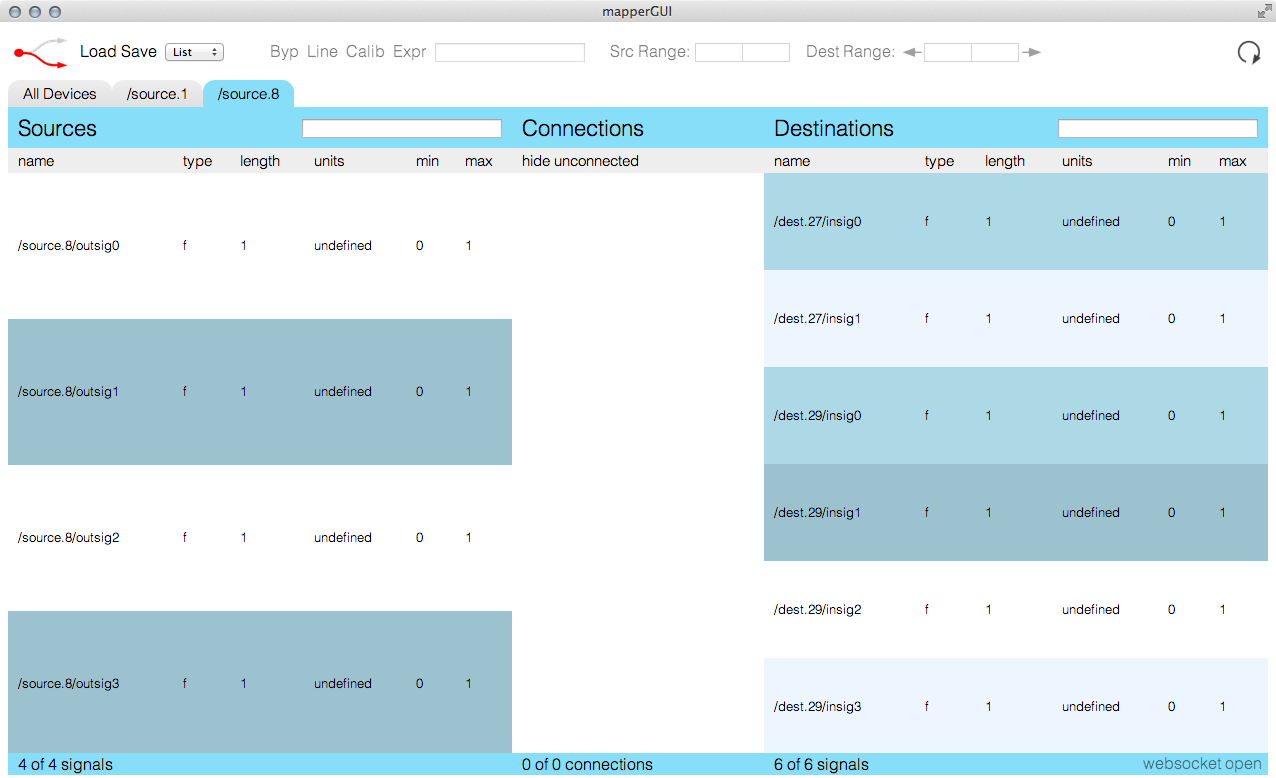
\includegraphics[width=\textwidth]{figures/multi-select_before_connect}
		\caption{Multiple rows selected}
		\label{fig:multiple_connect_before}
	\end{subfigure}
	\begin{subfigure}[]{0.49\textwidth}
		\centering
		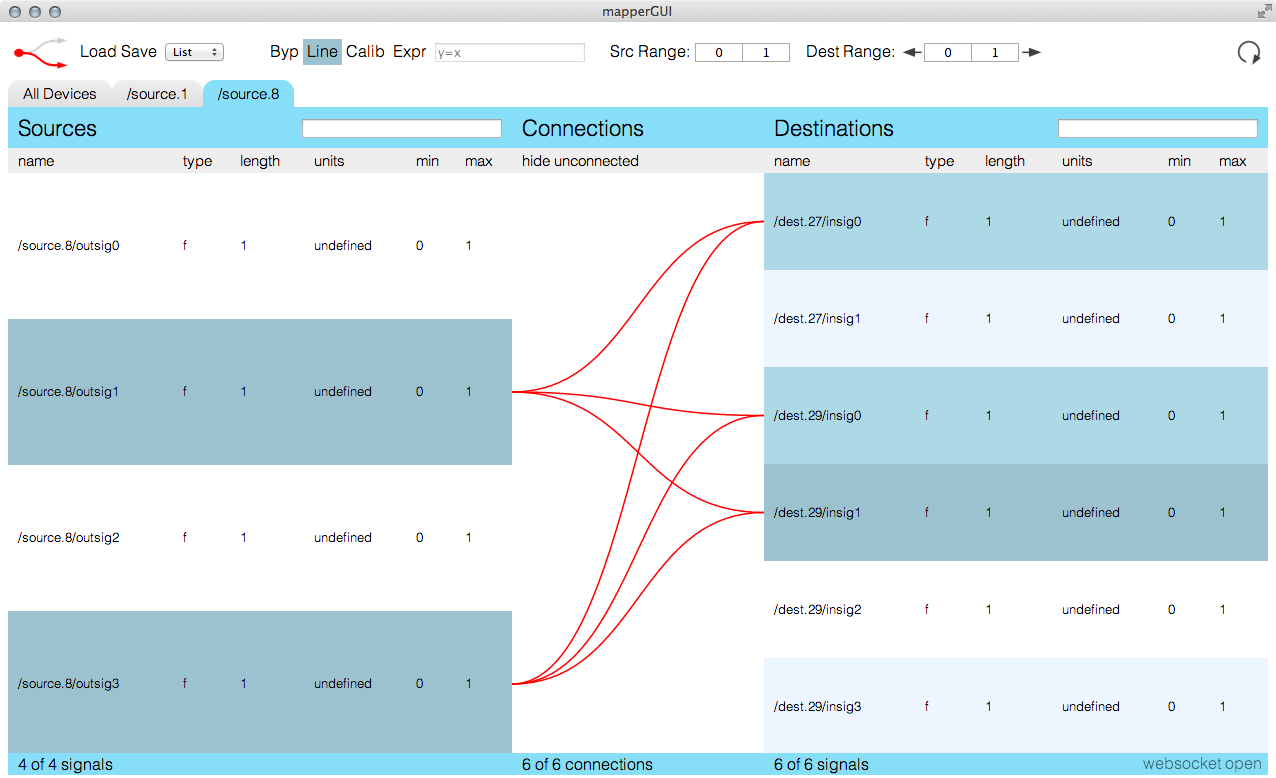
\includegraphics[width=\textwidth]{figures/multi-select_after_connect}
		\caption{After pressing the `c' key}
		\label{fig:multiple_connect_after}
	\end{subfigure}
	\caption{Simultaneous connection of multiple signals}\label{fig:multiple_connect}
\end{figure}

Users can also depress the ``shift'' key to select multiple rows simultaneously, a functionality common in other list interfaces ,like the Windows and Macintosh file browsers. Clicking anywhere in the container, except for the tables, de-selects all currently selected rows and arrows.
	
	% subsection multiple_selection (end)

	\subsection{Accommodating varying window sizes} % (fold)
	\label{sec:accomodating_sizes}

\begin{figure}
	\centering
	\begin{subfigure}[]{\textwidth}
		\centering
		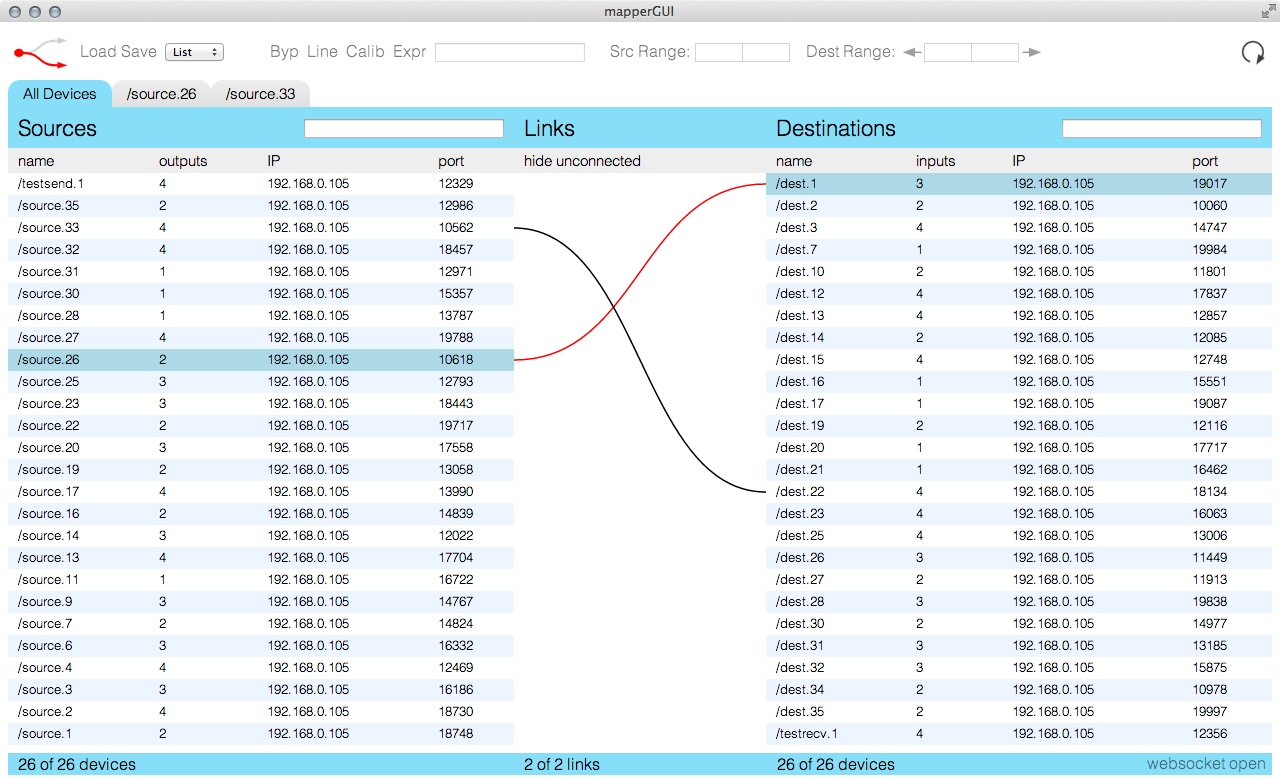
\includegraphics[width=\textwidth]{figures/before_resize_1280x760}
		\caption{List view at 1280 x 760 pixels}
		\label{fig:before_resize}
	\end{subfigure}
	\begin{subfigure}[]{0.5\textwidth}
		\centering
		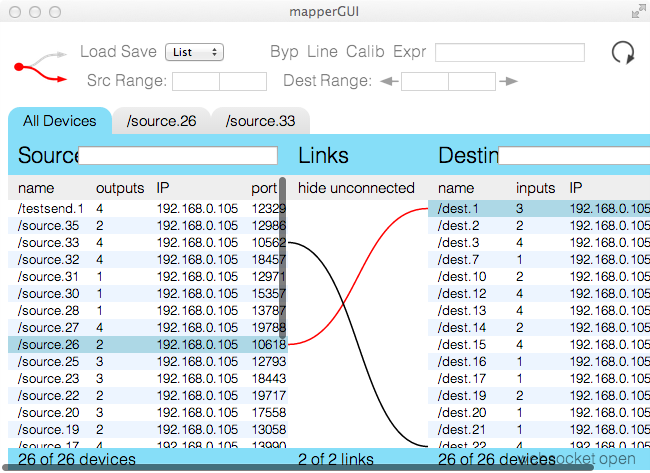
\includegraphics[width=\textwidth]{figures/after_resize_650x450}
		\caption{Same view resized to 650 x 450 pixels}
		\label{fig:after_resize}
	\end{subfigure}
	\caption{Resizing the ListView window. Rows condense, scroll bars appear and the top menu collapses in the smaller version.}\label{fig:resizing}
\end{figure}

One notable shortcoming of the Maxmapper GUI is inability to resize the application window. This creates problems for users with small screens, or those who would like to run Maxmapper side-by-side with other applications. MapperGUI can be resized in the same fashion as any other application, supporting windows as small as 100 x 124 pixels (about 3cm x 3cm).\footnote{All physical screen sizes quoted in this section are for a 96 pixel-per-inch hi-res display. Lower resolution displays will result in larger windows.}

Upon resizing, the size and shape of various on-screen elements change dynamically to fit the new window size (see figure \ref{fig:resizing}). The two device/signal tables always occupy two-fifths of the container area each, with the central canvas filling the remaining fifth. The container itself fills the entire window not occupied by the top bar. It will expand to fill any size, but has a programmed minimum height of 150 pixels (about 4cm) and minimum width of 700 pixels (about 18cm). Upon hitting these minimum dimensions, the GUI adds scroll bars to allow the user to view the entire display. Elements within the top menu fold onto multiple lines to accommodate narrower windows.


Maxmapper table rows have constant height. Unless many devices or signals are present large parts of the display are often empty. ListView instead calculates table elements to fill the available space, as can be seen in most of the figures of this chapter. Minimum row heights are set to 17 pixels. Once there is not enough space to accommodate all necessary rows, MapperGUI adds a scroll bar to the appropriate table. 

	% subsection accomodating_sizes (end)

	\subsection{Visual Redesign} % (fold)
	\label{sec:visual_redesign}

Keeping in line with visual guidelines summarized in section \ref{sec:data_viz}, we overhauled the look of the Webmapper interface to reduce visual noise, make better use of color and generally improve its aesthetic appeal. 

\begin{figure}[h]
\centering
	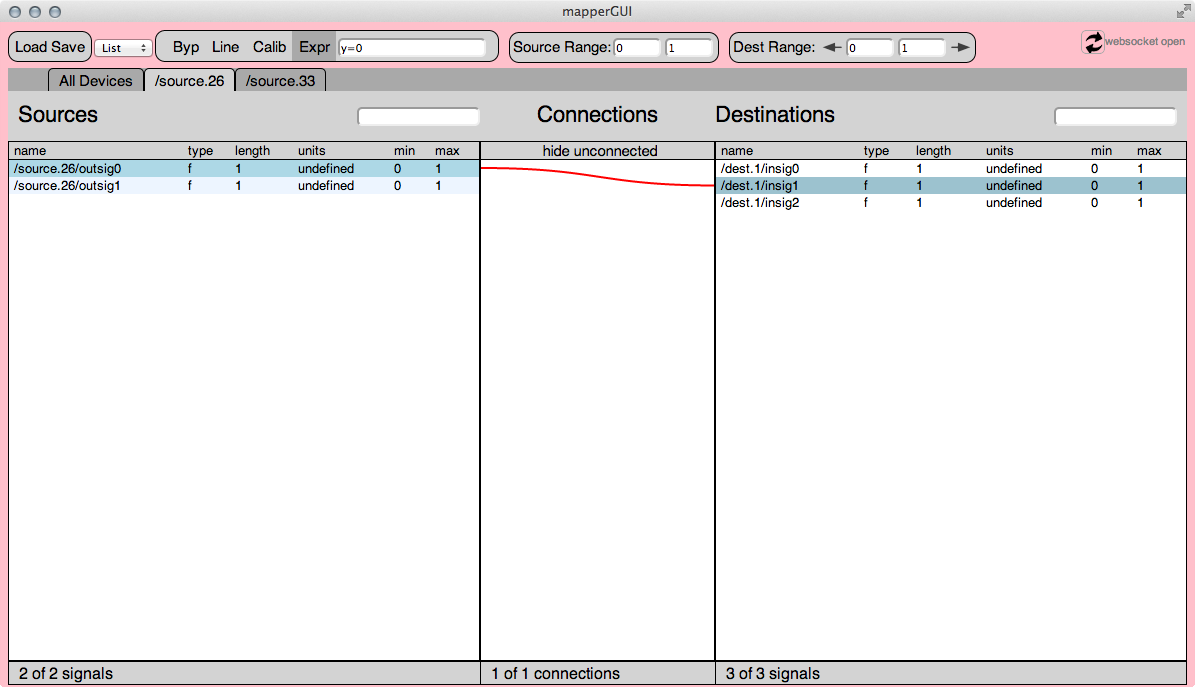
\includegraphics[width=\textwidth]{figures/before_redesign}
\caption{The list view before visual re-design}
\label{fig:before_redesign}
\end{figure}

First, much of the display area was wasted for simple networks, leading to the dynamic row sizing described above. The display was plagued by $1 + 1 = 3$ noise, causing negative space like the central canvas to attract the eye and making the display seem much more complex than necessary. All black borders were removed and font weight was lightened for all text, drastically reducing visual noise. Arrows now display with one-half of the stroke weight. This too reduces visual clutter and also differentiates arrows that are in the process of being drawn.

The pink background, though whimsical and popular at IDMIL, was deemed too bright to be used effectively over such a large area. It also distracted from the red color used to highlight selected connections and links. A neutral white was selected for the background, both to blend with input areas and to cause more contrast with row striping and highlights. Aside from the red for selected arrows, all colors are now a variation of an unobtrusive gray-blue. This contributes to the visual uniformity of the display, but also allows us to make visual distinctions between odd rows, even rows, selected rows, table headers and table footers without using borders.

Finally, a logo was added to the upper left-hand corner of the display. The logo is a simplified version of the overall libmapper logo\footnote{Can be seen at \url{www.libmapper.org}} with a white background. The red highlight color is maintained to match highlighted links and connections.

	% subsection visual_redesign (end)

	\subsection{Alternate views} % (fold)
	\label{sec:alternate_views}

Jon Wilansky, a fellow master's student at IDMIL, created two new views for MapperGUI. These took advantage of the new MVC architecture for the program. With these views in place it finally became possible to test our foundational hypothesis that a variety of displays would aid in mapping tasks.

		\subsubsection{GridView}

\begin{figure}[ht]
\centering
	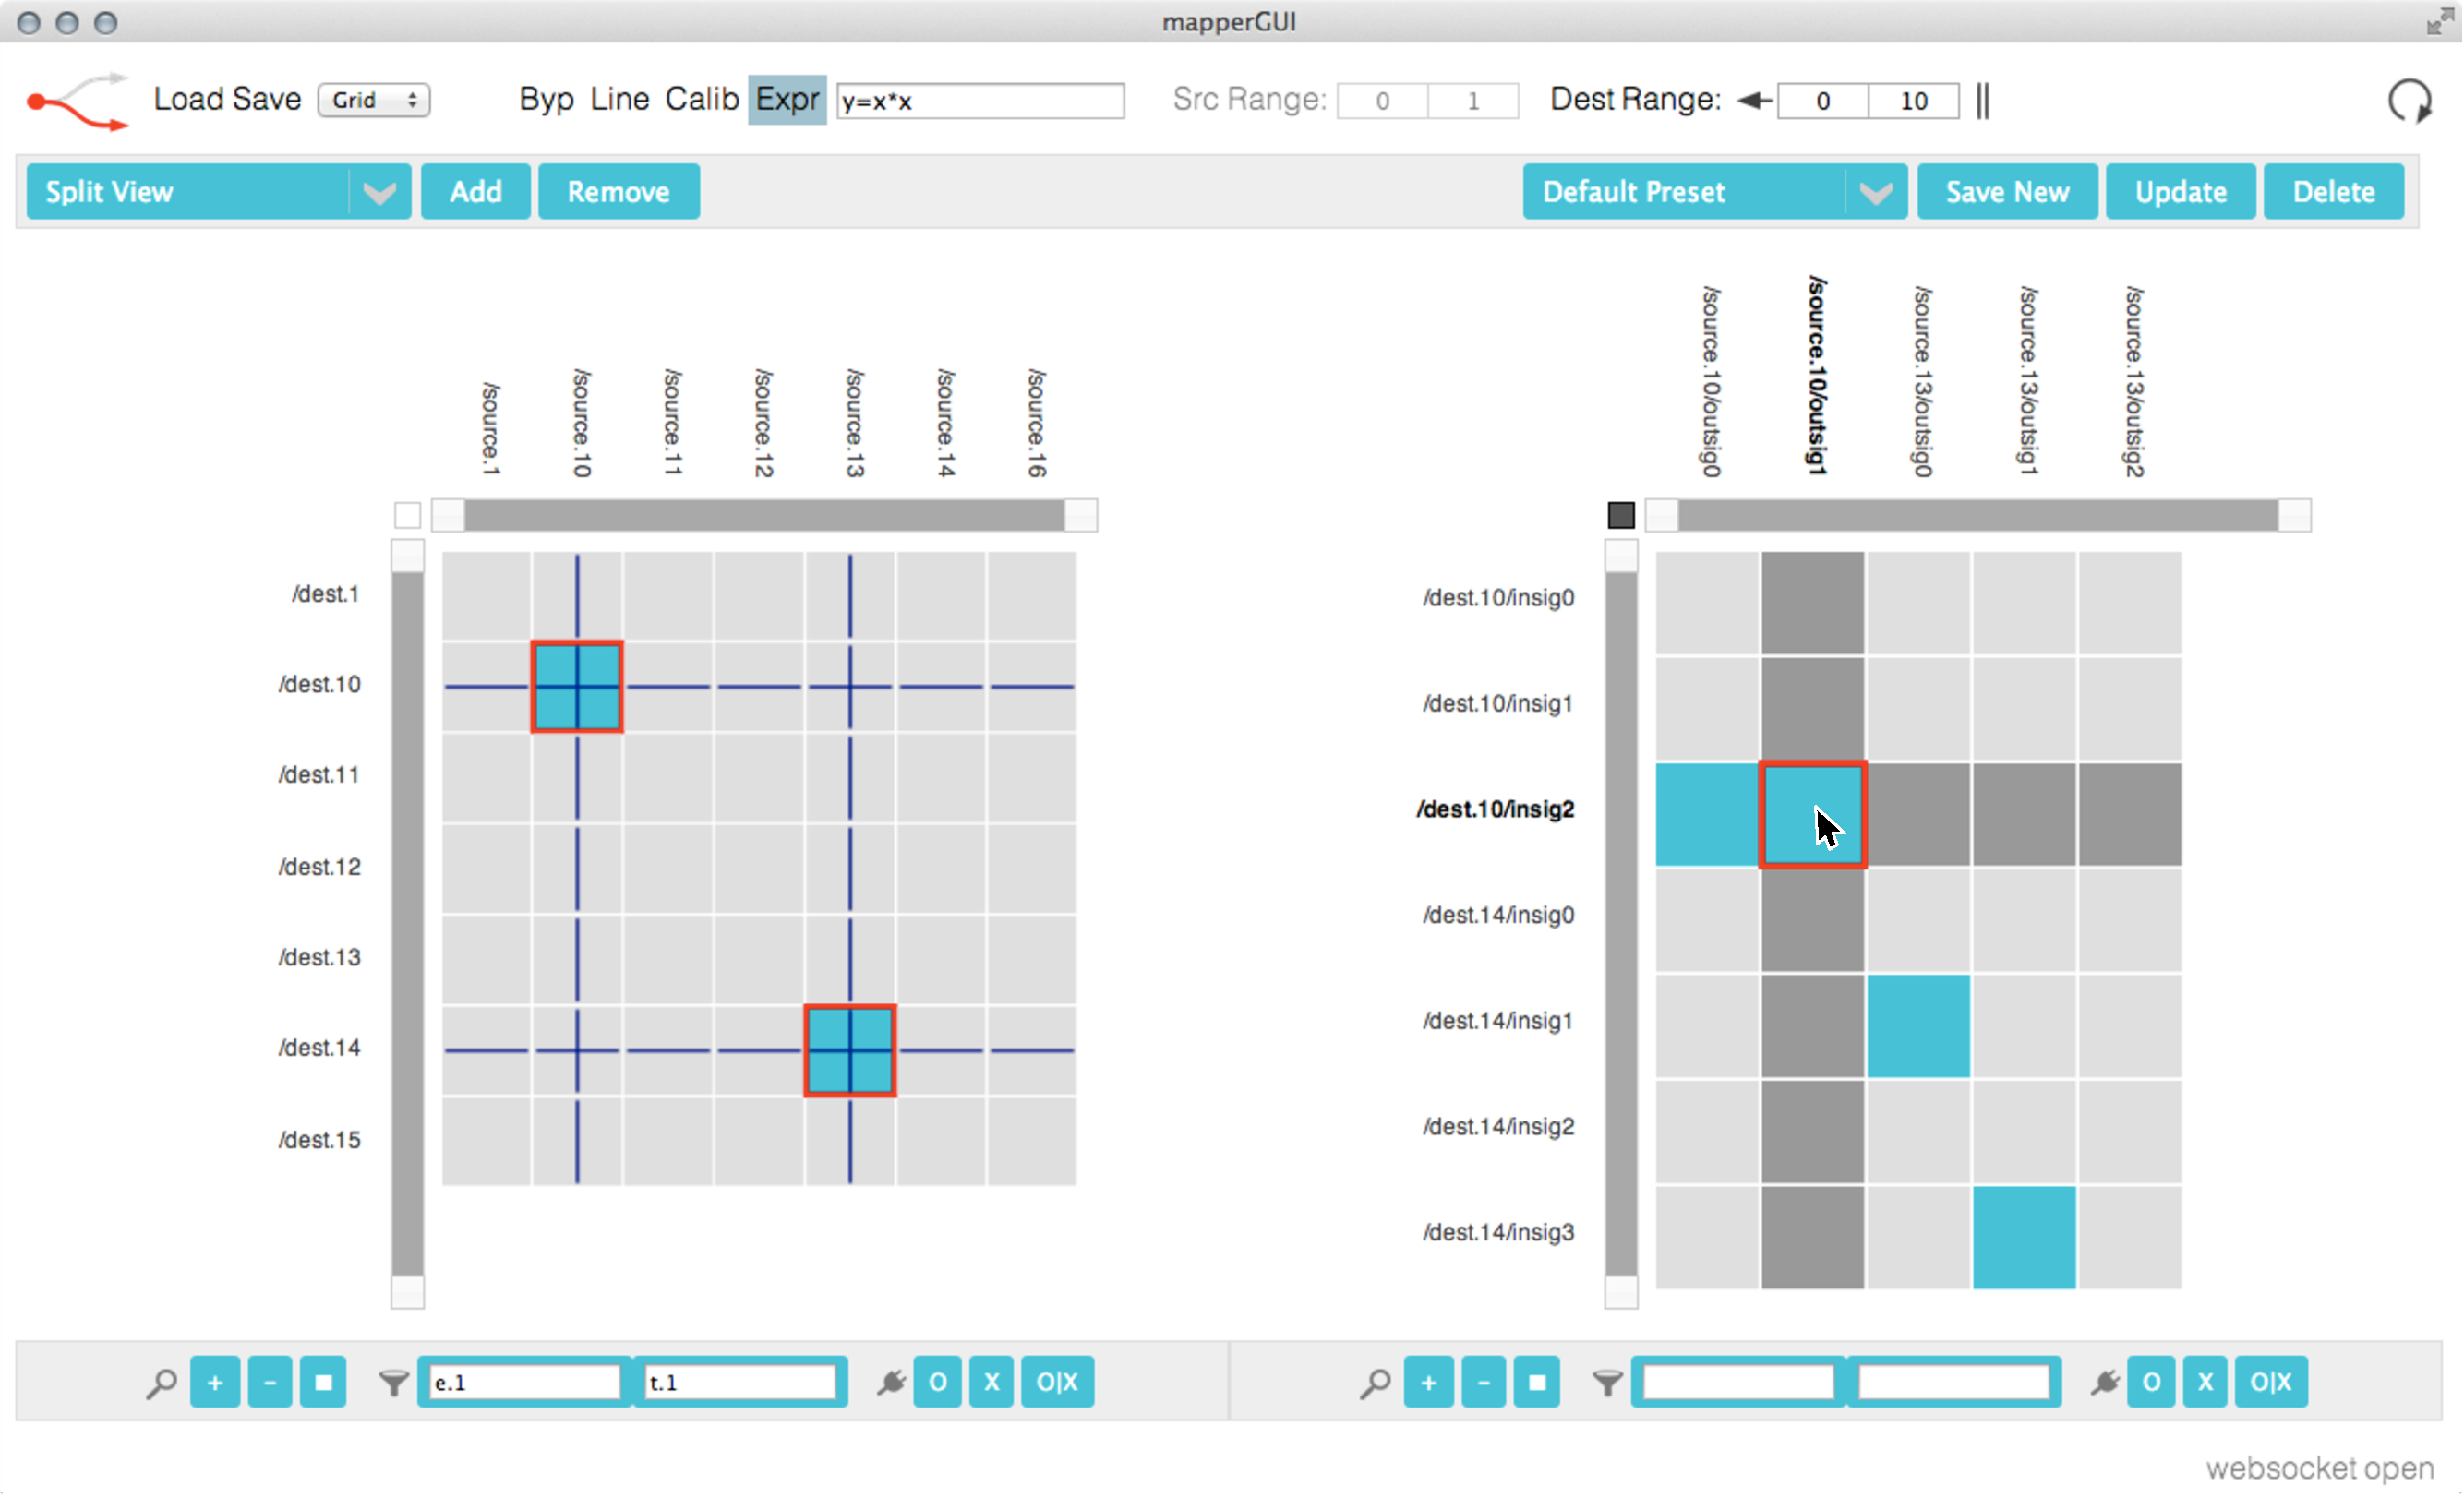
\includegraphics[width=\textwidth]{figures/grid_w_cursor}
\caption{GridView}
\label{fig:grid}
\end{figure}

First programmed and implemented was the ``grid'' view. The network is represented with two $m$-by-$n$ grids. The leftmost grid lists source devices horizontally and destination devices vertically. Links are formed by clicking on the square at the intersection between the desired source and destination devices. The second grid represents signals and connections. Signals must be explicitly added to this grid from the device grid by selecting the intersection and clicking add, or by pressing the ``a'' key. 

Both grids are fully filterable using text input fields below, which borrow code from ListView. Grids are also zoom-able using the endpoints of the scroll bars. Either grid can be hidden, allowing the user to focus the entire display on a single grid. Because this view is more customizable than ListView, the designer added an option to save view settings, causing GridView to remember which devices have been added to the signal grid.

GridView provides visual feedback by highlighting the associated row and column when the user places the cursor over a grid intersection. Text of the relevant devices/signals is also highlighted in this situation. Colors are designed to match the gray-blue style in ListView, hopefully creating the feel of a unified interface for MapperGUI. GridView highlights selected grid squares with the same red color as used in ListView and the logo.

The top bar looks and functions in the exact same fashion for GridView as in ListView. MVC architecture allows us to create modular view-control elements like this to be used with a variety of other view-controller pairs.

	\subsubsection{HiveView}

\begin{figure}[ht]
\centering
	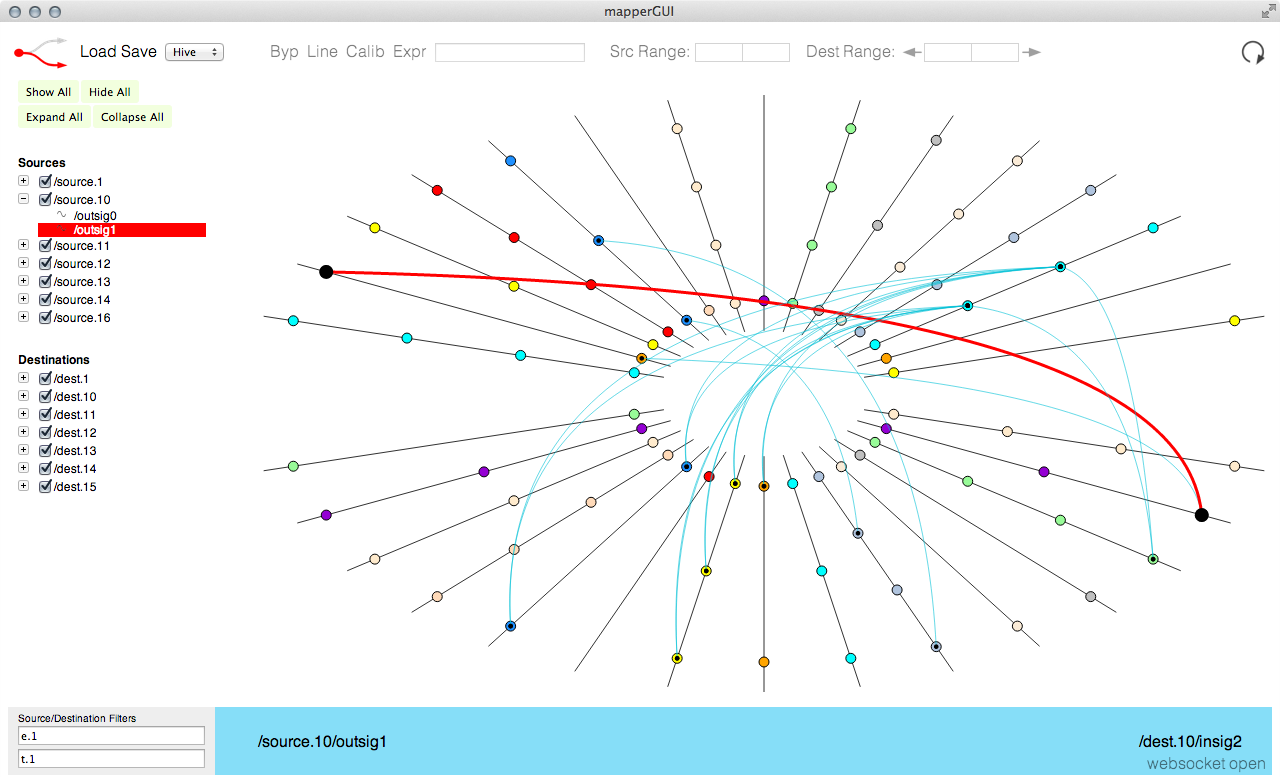
\includegraphics[width=\textwidth]{figures/hive}
\caption{HiveView}
\label{fig:hive}
\end{figure}
	
The ``hive'' view attempts to address the problem of visualizing entire networks simultaneously. This visualization borrows many techniques from Vizmapper (see section \ref{sub:vizmapper}). Solid black lines emanating from the center of the view signify network devices. Small circles representing child signals are distributed throughout each line. Thin blue curves flow between these circles, signifying connections. 

On the left side of HiveView, a menu displays expandable and collapsible list of all network devices. Expanded entries in this list display child signals. Connection lines highlight to red when clicked, and the bottom bar (colored our standard blue) presents the names of the connected signals. Placing the mouse cursor over device lines highlights all connections to that device. The same is true for mousing over individual signals or any item in the list on the left.

A text filter in the bottom right can narrow down the number of blue connection lines, though the black device lines and signal bubbles persist. Connection lines can also be hidden by toggling check-boxes to the left of items in the device list on the left.

As of the writing of this thesis HiveView is not yet as fully interactive as the other two views. It is not possible form connections or links by any means, though a dragging-type interaction like in ListView would be most desirable. It is possible to modify selected connections using the top toolbar, as the MVC structure preserves this functionality across views.

	% subsection alternate_views (end)

% section extension_of_control_and_visual_elements (end)

%%%%%%%%%%%%%%%%%%%%%%%%%%%%%%%%%%%%%%%%%%%%%%%%%%%%%%%%%%%%%%%%%%%%%%%%%%%%%%%%%%%%%%%%%%%%%%%%%%%%%%%%%%%%%%%%%%%%%%%%%%%%%%%%%%%%%%%%%%%%%%%%%%%%%%%%%%%%%%%%%%%%%%%%%%%%%%%%%%%%%%%%%%%%%%%%%%%%%%%%%%%%%%%%%%%%%%%%%%%%%%%%%%%%%%%%%%%%%%%%%%%%%%%%%%%%%%%%%%
\section{Other GUI features} % (fold)
\label{sec:other_gui_features}

	\subsection{Saving \& Loading} % (fold)
	\label{sec:saving_and_loading}

Saving and loading presents an interesting problem for libmapper networks.  Upon clicking the ``save'' button, connection information is serialized into a JSON\footnote{JavaScript Object Notation. A human-readable data-interchange format. [Online]. Available: \url{www.json.org}. Accessed July 30, 2013} file which the user is asked to name. Only visible connections, ones that are present in the selected tab in ListView, are recorded to the save file. Saving is not yet fully supported for GridView or HiveView.

A ``na\"{i}ve'' interpretation of loading mappings is implemented here. Though device information is encoded into the save file, it is not considered in the loading process. Mappings are loaded for all applicable signals. For example, in the following situation:

\begin{itemize}
	\item Devices \url{tstick.1}, \url{tstick.2} and \url{granul8.1} all exist on the network
	\item Both \url{tstick.1} and \url{tstick.2} have child signals named \url{raw/accelerometer/1/x} (they both should, as they are both t-sticks)
	\item A mapping is loaded that contains a connection \url{tstick.1/raw/accelerometer/1/x} $\rightarrow$ \url{granul8.1/filter/envelope/frequency/low}
\end{itemize}

For the above case the single connection will be loaded for \emph{both} t-sticks, creating two total connections to \url{granul8.1}'s low filter envelope. If two instances of the granul8 synthesizer exist, then the connection will be loaded four times, one for each iteration of t-stick $\rightarrow$ granul8.

This na\"ive implementation is used to maintain a modularity for mappings, such that similar devices and equivalent devices with different names can share mappings. This makes sense for libmapper networks, as they are ideally collaborative and ordinal numbers appearing after device names are arbitrary. 
	
	% subsection saving_&_loading (end)

	\subsection{Creation of a standalone \& distribution} % (fold)
	\label{sec:creation_of_a_standalone_and_distribution}
	
Though it is already in use, we would like for MapperGUI to be quickly be adopted by a greater number of users. This would assist us in debugging and improving the interface. It would also hopefully bring a new set of users to libmapper itself, encouraging use of the API and its implementation into new DMIs. Unfortunately, to get libmapper and MapperGUI up and running from the source code requires installing package management software and compiling multiple dependencies. This is rather time-consuming and well beyond what should be expected of a non-programmer. 

To aid in ease-of-use and adoption, we compiled a ``standalone'' version of MapperGUI. It is presently available for free download at \url{www.libmapper.org/downloads} under the name Webmapper\footnote{The name will be officially changed once Maxmapper has been phase out completely.}. The standalone includes libmapper code, and thus can be run on a machine that does not have libmapper explicitly installed. To the user it looks like any other Macintosh application: an icon on which to double-click.

The current version is still very much in test phase, and includes a readme file describing likely bugs, and the non-ideal startup method.\footnote{Running the program and navigating to \url{localhost:50000} in the Google Chrome browser.} It presently supports Macintosh OSX only, though Linux and Microsoft Windows releases are planned.

	% subsection creation_of_a_standalone_&_distribution (end)

% section other_gui_features (end)




